% Provenance (never printed): old terminale S material on magmatism in
% subduction zones (volcanic arcs above the slab, water released by the slab
% and hydrous melting of the mantle wedge, andesitic volcanism and granitoid
% plutons, growth of the continental crust). Owner (Sync 0): volcanic arc,
% hydrous melting, granodiorite, batholith, continental growth. Subduction,
% slab, Wadati-Benioff zone, blueschist and eclogite are g11.06's; partial and
% decompression melting and peridotite g11.05's; andesite, diorite, rhyolite,
% pluton g11.08's; continental crust g12.01's; magma, explosive eruption Book 1's
% (g7): recalled, never redefined. Figures: figdata/grade-12/arc_magmatism.py
% (GVP volcanoes, ComCat NE Japan band, dry solidus via grade-11
% geotherm_solidus.py, wet solidus brackets of Wang 2020 and Kawamoto-Holloway 1997).
\chapter{El magmatismo de las zonas de subducción}\label{ch:g12:subduction-magmatism}

El 18 de mayo de 1980, a las 8:32 de la mañana, un terremoto de magnitud 5.1
sacudió el monte Santa Helena. Al instante, el flanco norte del volcán, que se
había ido abombando hacia fuera unos dos metros al día, se deslizó: la mayor
avalancha de derrubios de la historia registrada, unos \qty{2.5}{km^3} de
roca. Liberado de su carga, el magma rico en gas del interior salió disparado
de lado a través de la cicatriz, a no menos de \qty{480}{km/h}, y arrasó los
bosques en \qty{600}{km^2}. En quince minutos, una columna de ceniza se
elevaba a más de \qty{24}{km}, y la erupción duró nueve horas. Sesenta y una
personas murieron o nunca fueron encontradas.
% ledger: usgs:b2-msh-1980, usgs:msh-deaths

\begin{omfigure}
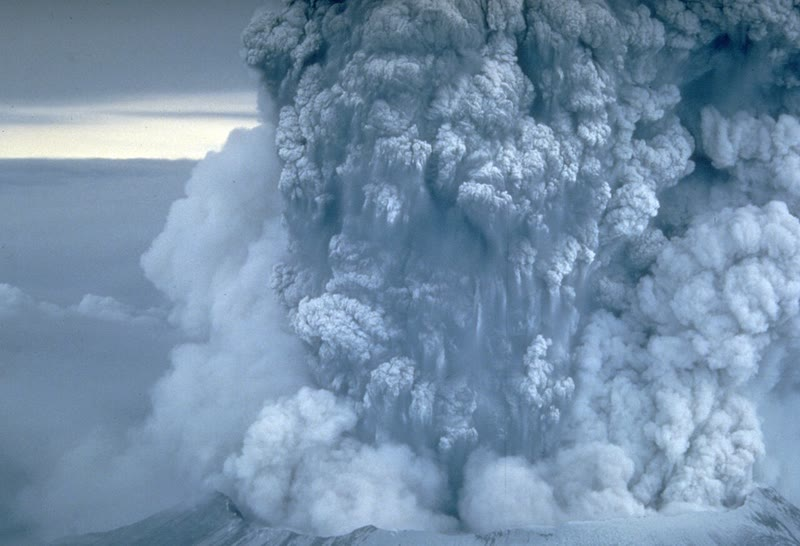
\includegraphics[width=0.55\linewidth]{images/book2/g12-swanson-st-helens-plume.jpg}

{\small La columna de ceniza del monte Santa Helena el 18 de mayo de 1980,
que se elevó a más de \qty{24}{km} en menos de quince minutos. Fotografía de
Donald A.~Swanson, USGS (dominio público).}
\end{omfigure}
% ledger: photo:g12-st-helens, usgs:b2-msh-1980

El monte Santa Helena forma parte de una línea de volcanes ---Baker, Rainier,
Hood, Shasta y otros--- que se alza sobre el lugar donde una pequeña placa
oceánica, la placa de Juan de Fuca, se hunde bajo América del Norte. Este
capítulo se pregunta por qué hay volcanes allí, por qué sus erupciones son tan
a menudo violentas y qué ocurre con el magma que nunca llega a la superficie.
% ledger: earle:cascades

\begin{recall}
En una \omterm{def:g11:subduction-zones:subduction}{zona de subducción}, una placa de \omterm{def:g11:ocean-ridges:oceanic-lithosphere}{litosfera oceánica} se hunde de nuevo
en el manto bajo otra placa; sus terremotos, la \omterm{def:g11:subduction-zones:benioff}{zona de Wadati--Benioff},
dibujan la \omterm{def:g11:subduction-zones:slab}{losa} hasta profundidades de \qty{670}{km}
(el \cref{ch:g11:subduction-zones}). El manto está formado por \omterm{def:g11:ocean-ridges:peridotite}{peridotita}; es
sólido, pero una roca que asciende y queda menos comprimida puede fundirse en
parte, por \omterm{def:g11:ocean-ridges:partial-melting}{fusión por descompresión}, como bajo una dorsal (el
\cref{ch:g11:ocean-ridges}). La \omterm{def:g11:igneous-rocks:rock-names}{andesita} es una \omterm{def:g11:igneous-rocks:volcanic-plutonic}{roca volcánica} \omterm{def:g11:igneous-rocks:felsic-mafic}{intermedia}
entre el basalto y la \omterm{def:g11:igneous-rocks:rock-names}{riolita}; la \omterm{def:g11:igneous-rocks:rock-names}{diorita} es su equivalente plutónico, y un
\omterm{def:g11:igneous-rocks:intrusion}{plutón} es un gran cuerpo de magma que se enfrió bajo tierra
(el \cref{ch:g11:igneous-rocks}). La \omterm{def:g12:continental-crust:continental-crust}{corteza continental} es gruesa y ligera,
formada sobre todo por roca granítica en su parte superior (el
\cref{ch:g12:continental-crust}). Una erupción explosiva hace estallar el
magma en fragmentos con su propio gas (Libro 1, año 7).
\end{recall}
% ledger: tulane:magma-types, tulane:intrusions, rg14:crust

\section{Los arcos volcánicos}

La mayoría de los volcanes activos en tierra firme no se sitúan al azar. De
los 1214 volcanes que han entrado en erupción desde el final de la última
glaciación y figuran en el catálogo del Global Volcanism Program, 838 ---más
de dos de cada tres--- se alzan sobre una \omterm{def:g11:subduction-zones:subduction}{zona de subducción}. Alrededor del
Pacífico forman un anillo casi continuo, a menudo llamado Cinturón de Fuego, y
cada una de sus líneas corre paralela a una fosa, del lado de la placa que no
se hunde.
% values: n_volcanoes 1214, n_subduction 838, frac_subduction 0.690 (arc_magmatism.py)
% ledger: data:gvp, tulane:arc

\begin{omfigure}
\begin{tikzpicture}
\begin{axis}[ommap, width=\linewidth, xtick={-180,-90,...,180}, ytick={-60,0,60},
  legend style={font=\scriptsize, at={(0.5,-0.13)}, anchor=north, legend columns=3,
    /tikz/every even column/.append style={column sep=6pt}}]
\addplot[fill=omLithAlluv, draw=black!45, line width=0.2pt, forget plot] table {figdata/out/shared-geo-land.dat};
\addplot[black!70, line width=0.5pt, forget plot] table {figdata/out/shared-geo-school-subduction.dat};
\addplot[fill=black!70, draw=none, forget plot] table {figdata/out/shared-geo-school-teeth.dat};
% computed in figdata/grade-12/arc_magmatism.py; ledger: data:gvp, data:pb2002, data:ne-land
\addplot[only marks, mark=triangle*, mark size=1.1pt, black!40] table[x=lon, y=lat] {figdata/out/grade-12-arc_magmatism-world-other.dat};
\addplot[only marks, mark=triangle*, mark size=1.3pt, omThm] table[x=lon, y=lat] {figdata/out/grade-12-arc_magmatism-world-sub.dat};
\addlegendimage{black!70, line width=0.5pt}
\legend{{otros volcanes}, {volcanes sobre una zona de subducción}, {fosa}}
\end{axis}
\end{tikzpicture}

{\small Los volcanes activos desde el final de la última glaciación, en rojo
los que se alzan sobre una \omterm{def:g11:subduction-zones:subduction}{zona de subducción}, con las fosas (línea negra,
triángulos sobre la placa cabalgante). Datos: Smithsonian Global Volcanism
Program; límites de placas de Bird (2003); tierras de Natural Earth.}
\end{omfigure}
% values: n_subduction 838 of 1214 (arc_magmatism.py)

\begin{definition}[Arco volcánico]\label{def:g12:subduction-magmatism:arc}
Un \emph{arco volcánico}\index{arco volcanico@arco volcánico} es una línea de
volcanes sobre la placa cabalgante de una \omterm{def:g11:subduction-zones:subduction}{zona de subducción}, paralela a la
fosa, situada sobre el lugar donde la \omterm{def:g11:subduction-zones:slab}{losa} ha alcanzado una profundidad de
unos cien kilómetros. Es un \emph{arco insular} cuando surge del fondo
marino, como en Japón o Indonesia, y un arco continental cuando se alza sobre
un continente, como en los Andes o las Cascadas.
\end{definition}
% ledger: tulane:arc, earle:arc-water, earle:cascades, sa06:slab-depth

El borde del arco más cercano a la fosa se llama \textbf{frente volcánico}:
del lado de la fosa no hay ningún volcán. ¿A qué profundidad está la \omterm{def:g11:subduction-zones:slab}{losa}
bajo él?

\begin{proposition}[La losa bajo el frente volcánico]\label{prop:g12:subduction-magmatism:depth}
Si la \omterm{def:g11:subduction-zones:slab}{losa} es un plano que buza un ángulo $\theta$ a partir de la fosa, y el
frente volcánico está a una distancia horizontal $d$ de la fosa, entonces el
techo de la \omterm{def:g11:subduction-zones:slab}{losa} se encuentra bajo el frente a una profundidad
\[
  H = d \tan\theta .
\]
\end{proposition}

\begin{proof}
Toma un corte vertical perpendicular a la fosa. La \omterm{def:g11:subduction-zones:slab}{losa}, la superficie y la
vertical bajo el frente forman un triángulo rectángulo, con el ángulo recto
bajo el frente: el lado a lo largo de la superficie es $d$, el lado vertical
es $H$, y el ángulo en la fosa es $\theta$. Así que $\tan\theta = H/d$.
\end{proof}

Una recopilación de 839 centros volcánicos a lo largo de \qty{33000}{km} de
arcos midió $H$ bajo cada uno de ellos: promediada sobre tramos de arco de
\qty{500}{km}, va de 72 a \qty{173}{km}, con una media de \qty{105}{km}. Los
arcos situados sobre \omterm{def:g11:subduction-zones:slab}{losas} muy inclinadas están cerca de su fosa, y los
situados sobre \omterm{def:g11:subduction-zones:slab}{losas} de buzamiento suave, lejos de ella, pero la \omterm{def:g11:subduction-zones:slab}{losa} que
tienen debajo está siempre a unos cien kilómetros de profundidad.
% ledger: sa06:slab-depth

\begin{method}[Encontrar la losa bajo un volcán]\label{met:g12:subduction-magmatism:slab}
\begin{enumerate}
  \item Toma los terremotos de una franja estrecha perpendicular al arco, y
        representa su profundidad frente a su distancia a lo largo de ella, a
        escala real.
  \item Quédate con los terremotos de más de unos \qty{70}{km} de
        profundidad: los más someros se producen también en la placa
        cabalgante y en la falla entre las dos placas.
  \item Traza la línea, o lee la profundidad, de los terremotos profundos bajo
        el frente volcánico: esa es la profundidad de la \omterm{def:g11:subduction-zones:slab}{losa} allí.
  \item Compruébalo con $H = d\tan\theta$, midiendo $d$ desde la fosa y el
        buzamiento $\theta$ en el corte.
\end{enumerate}
\end{method}

\begin{omfigure}
\begin{tikzpicture}
\begin{axis}[omsection, name=jp, scale only axis, width=0.8\linewidth, height=0.2857\linewidth,
  xmin=0, xmax=700, ymin=0, ymax=250, y dir=reverse,
  xlabel={distancia al este de \ang{138}~E (\unit{km})}, ylabel={profundidad (\unit{km})},
  xtick={0,100,...,700}, ytick={0,50,...,250}, tick label style={font=\small},
  every axis label/.append style={font=\small}]
% computed in figdata/grade-12/arc_magmatism.py; ledger: data:b2-usgs-ne-japan, data:gvp, data:pb2002
\addplot[only marks, mark=*, mark size=0.55pt, black!35] table[x=x_km, y=depth] {figdata/out/grade-12-arc_magmatism-jp-quakes.dat};
\addplot[omDef, line width=0.9pt, dashed] table[x=x_km, y=depth] {figdata/out/grade-12-arc_magmatism-jp-slab.dat};
\addplot[only marks, mark=triangle*, mark size=2.6pt, omThm] table[x=x_km, y expr=-7] {figdata/out/grade-12-arc_magmatism-jp-volc.dat};
\draw[omThm, densely dotted, line width=0.8pt] (axis cs:259.2,0) -- (axis cs:259.2,98.2);
\fill[omThm] (axis cs:259.2,98.2) circle (1.6pt);
\coordinate (front) at (axis cs:259.2,-14);
\coordinate (trench) at (axis cs:528.9,-14);
\coordinate (H) at (axis cs:262,60);
\coordinate (slab) at (axis cs:95,228);
\draw[black, line width=0.9pt] (axis cs:528.9,-12) -- (axis cs:528.9,0);
\end{axis}
\node[font=\scriptsize, anchor=south, text=omThm] at (front) {frente volcánico (Iwate)};
\node[font=\scriptsize, anchor=south] at (trench) {fosa de Japón};
\node[font=\scriptsize, anchor=west, text=omThm, fill=white, inner sep=1pt] at (H) {\qty{98}{km}};
\node[font=\scriptsize, anchor=west, text=omDef, fill=white, inner sep=1pt] at (slab) {losa, con un buzamiento de unos \ang{20}};
\end{tikzpicture}

{\small Un corte a través del noreste de Japón a escala real: los terremotos
de magnitud 4.5 o más entre \ang{37.5} y \ang{40.5}~N, 1976--2025 (en gris),
los volcanes de la misma franja (triángulos rojos) y la recta ajustada a los
terremotos de más de \qty{70}{km} de profundidad (azul, discontinua). Dos de
cada cinco sucesos someros al este de \ang{141.5}~E datan de 2011, el año del
gran terremoto de marzo. Datos: catálogo de terremotos del USGS; Smithsonian
Global Volcanism Program; límites de placas de Bird (2003).}
\end{omfigure}
% values: shallow (<70 km) events east of 141.5 E: 3622, of which 1451 in 2011 (0.40); ledger usgs:tohoku
% values: jp_front_lon 141.0 (x 259.2 km), jp_trench_lon 144.12 (x 528.9), jp_front_trench_km 269.4, jp_dip_deg 19.98, jp_H_geom 98.0, bin_141_median 98.15, jp_slab_depth_front 105.6 (arc_magmatism.py)

\begin{example}[El noreste de Japón]\label{ex:g12:subduction-magmatism:japan}
En la franja de la figura, el volcán situado más al este es el Iwate, a
\ang{141.0}~E, y la fosa de Japón está a \ang{144.1}~E. Un grado de longitud
mide allí $111.2\cos\ang{39} \approx \qty{86.4}{km}$, así que $d \approx 3.12 \times 86.4
\approx \qty{270}{km}$. Los terremotos profundos buzan unos \ang{20}, y
\[
  H = 270 \times \tan\ang{20} \approx \qty{98}{km}.
\]
Los terremotos de más de \qty{70}{km} de profundidad que se encuentran bajo el
propio frente tienen una profundidad mediana de \qty{98}{km}: los dos valores
coinciden, cerca de la media mundial.
\end{example}
% values: km_per_deg_lon 86.415, jp_front_trench_km 269.4, jp_dip_deg 19.98, jp_H_geom 97.98, bin_141_median 98.15 (arc_magmatism.py)

\section{El agua funde el manto}

Bajo un arco, la \omterm{def:g11:subduction-zones:slab}{losa} está fría, y también lo está la \omterm{def:g11:ocean-ridges:oceanic-lithosphere}{corteza oceánica} que
lleva encima: no puede fundirse. El magma tiene que proceder del manto
caliente situado sobre la \omterm{def:g11:subduction-zones:slab}{losa}, la \textbf{cuña del manto}. Pero la cuña no
asciende, así que no puede fundirse por descompresión como bajo una dorsal.
Hay otra cosa que rebaja su temperatura de fusión: el agua.
% ledger: earle:settings (subducted crust stays cool), earle:flux-melting, earle:arc-water

La \omterm{def:g11:ocean-ridges:oceanic-lithosphere}{corteza oceánica} se empapa de agua de mar cerca de la dorsal donde se
forma, y gran parte de esa agua acaba encerrada en sus minerales, sobre todo
en la serpentina, formada a partir del olivino y el piroxeno de la corteza. A
medida que la \omterm{def:g11:subduction-zones:slab}{losa} se hunde y se calienta, esos minerales se descomponen y
liberan su agua. El agua asciende hacia la \omterm{def:g11:ocean-ridges:peridotite}{peridotita} caliente de la cuña que
hay encima.
% ledger: earle:arc-water, tulane:arc

\begin{definition}[Fusión hidratada]\label{def:g12:subduction-magmatism:hydrous-melting}
La \emph{fusión hidratada}\index{fusion hidratada@fusión hidratada} (o fusión por
aporte de agua) es la \omterm{def:g11:ocean-ridges:partial-melting}{fusión parcial} de una roca causada por la adición de
agua, que rebaja la temperatura a la que la roca empieza a fundirse.
\end{definition}
% ledger: earle:flux-melting, earle:arc-water

La temperatura a la que una roca empieza a fundirse, a una presión dada, es su
\textbf{solidus}. Para la \omterm{def:g11:ocean-ridges:peridotite}{peridotita} seca se conoce bien; con agua es mucho
más difícil de medir, y los valores publicados aún difieren entre 200 y
\qty{600}{\celsius}. Los experimentos más recientes lo sitúan entre 950 y
\qty{1000}{\celsius} a \qty{3}{GPa}, a unos \qty{95}{km} de profundidad, y
justo por encima de \qty{1000}{\celsius} de 5 a \qty{11}{GPa}. La \omterm{def:g11:ocean-ridges:peridotite}{peridotita}
seca a \qty{3}{GPa} solo empieza a fundirse hacia los \qty{1470}{\celsius}:
el agua rebaja el solidus unos \qty{500}{\celsius}.
% values: dry_T_3gpa 1473.4, dry_minus_wet_3gpa 498, z_3gpa_km 95.2, dry_minus_wet_5gpa 658 (arc_magmatism.py)
% ledger: hirschmann:solidus, wang20:wet-solidus, kh97:wet-solidus, data:prem, earth:gmean

\begin{omfigure}
\begin{tikzpicture}
\begin{axis}[omrecord, name=sol, scale only axis, width=0.62\linewidth, height=6.2cm,
  xmin=700, xmax=1900, ymin=0, ymax=230, y dir=reverse,
  xlabel={temperatura (\unit{\celsius})}, ylabel={profundidad (\unit{km})},
  xtick={800,1000,...,1800}, ytick={0,50,...,200}, axis y line*=left]
% computed in figdata/grade-12/arc_magmatism.py (dry: Hirschmann 2000 with PREM pressures; wet: Wang 2020, Kawamoto-Holloway 1997)
\addplot[omProp, line width=1.2pt] table[x=T_dry, y=depth_km] {figdata/out/grade-12-arc_magmatism-solidus.dat};
\addplot[omDef, line width=2.4pt] coordinates {(950,95.24) (1000,95.24)};
\addplot[omDef, line width=1.2pt] coordinates {(1000,155.6) (1000,216.3)};
\draw[-{Stealth}, black!70, line width=0.8pt] (axis cs:1460,95.24) -- (axis cs:1015,95.24);
\coordinate (gap) at (axis cs:1240,95.24);
\coordinate (dry) at (axis cs:1600,40);
\coordinate (wet) at (axis cs:1015,190);
\coordinate (wet3) at (axis cs:975,90);
\end{axis}
\begin{axis}[scale only axis, width=0.62\linewidth, height=6.2cm, at={(sol.south west)}, anchor=south west,
  xmin=700, xmax=1900, ymin=0, ymax=230, y dir=reverse, axis x line=none, axis y line*=right,
  axis line style={-}, ylabel={presión (\unit{GPa})},
  ytick={34.9,65.1,95.2,125.5,155.6,185.9,216.3}, yticklabels={1,2,3,4,5,6,7},
  every axis label/.append style={font=\small}, tick label style={font=\small}]
% pressure ticks at the PREM depths of 1-7 GPa (arc_magmatism.depth_at_pressure)
\end{axis}
\node[font=\scriptsize, anchor=south] at ([yshift=2pt]gap) {unos \qty{500}{\celsius}};
\node[font=\scriptsize, text=omProp, anchor=west, align=left] at (dry) {la peridotita\\seca empieza\\a fundirse};
\node[font=\scriptsize, text=omDef, anchor=west, align=left] at (wet) {con agua: justo por\\encima de \qty{1000}{\celsius}};
\node[font=\scriptsize, text=omDef, anchor=south] at ([yshift=2pt]wet3) {950--1000};
\end{tikzpicture}

{\small La temperatura a la que la \omterm{def:g11:ocean-ridges:peridotite}{peridotita} del manto empieza a fundirse,
frente a la profundidad: seca (naranja) y saturada de agua (azul, los dos
intervalos medidos hasta ahora). A la profundidad de la \omterm{def:g11:subduction-zones:slab}{losa} bajo los arcos,
unos \qty{100}{km}, el agua la rebaja unos \qty{500}{\celsius}. Fuentes:
Hirschmann (2000), con las densidades del PREM; Wang y otros (2020); Kawamoto
y Holloway (1997).}
\end{omfigure}
% values: dry_T_3gpa 1473.4, dry_T_100km 1489.4, P_100km_gpa 3.157 (arc_magmatism.py)

Así, el agua consigue lo que el calor por sí solo no podía: hace que se funda
parte de la cuña caliente. El magma, más ligero que el manto sólido que lo
rodea, asciende hacia la superficie; una parte entra en erupción, y mucha más
se queda y se enfría bajo tierra. El lugar donde se libera el agua, y donde la
cuña que hay encima está lo bastante caliente para fundirse una vez
humedecida, es lo que fija el frente volcánico unos cien kilómetros por encima
de la \omterm{def:g11:subduction-zones:slab}{losa}.
% ledger: earle:arc-water, tulane:arc, sa06:slab-depth, wang20:wet-solidus (position of the volcanic front controlled by melting in the wedge)

\begin{omfigure}
\begin{tikzpicture}[x=1cm, y=1cm, font=\scriptsize]
  % mantle
  \fill[omLithPeridotite!45] (0,-0.9) -- (7.4,-0.9) -- (7.5,-0.85) -- (6.5,-1.6) -- (5.5,-2.6) -- (4.5,-3.8)
    -- (4.25,-4.3) -- (0,-4.3) -- cycle;
  % sea and overriding continental crust
  \fill[omSea] (8.0,0) -- (12,0) -- (12,-0.4) -- (8.5,-0.4) -- cycle;
  \fill[omLithGranite!55] (0,0.1) -- (8.0,0.1) -- (8.5,-0.4) -- (7.5,-0.85) -- (7.4,-0.9) -- (0,-0.9) -- cycle;
  % the slab
  \fill[omLithBasalt!45, draw=black!60] (12,-0.4) -- (8.5,-0.4) -- (7.5,-0.85) -- (6.5,-1.6) -- (5.5,-2.6) -- (4.5,-3.8)
    -- (4.25,-4.3) -- (5.15,-4.3) -- (5.2,-4.3) -- (6.15,-3.15) -- (7.1,-2.2) -- (8.0,-1.55) -- (8.9,-1.2) -- (12,-1.2) -- cycle;
  \node at (10.4,-0.8) {litosfera oceánica};
  \node[anchor=west] at (6.0,-3.4) {losa que se hunde};
  % melting in the wedge, rising magma, plutons, volcano
  \fill[omThm!35, draw=omThm, densely dashed] (5.2,-1.75) ellipse (0.6 and 0.3);
  \node[omThm] at (5.2,-1.75) {fusión};
  \foreach \y in {-1.3,-1.05} \fill[omThm!80] (5.2,\y) circle (0.07);
  \fill[omLithGranite, draw=black!60] (4.75,-0.55) ellipse (0.42 and 0.2);
  \fill[omLithGranite, draw=black!60] (5.65,-0.4) ellipse (0.32 and 0.16);
  \node[anchor=east] at (4.25,-0.55) {plutones};
  \draw[omThm, line width=1pt] (5.2,0.1) -- (5.2,-0.85);
  \fill[black!65] (4.75,0.1) -- (5.2,0.75) -- (5.65,0.1) -- cycle;
  \node[anchor=south] at (5.2,0.8) {volcán};
  % water released by the slab
  \foreach \x/\y in {6.5/-1.6, 6.0/-2.1, 5.6/-2.5}
    \draw[omDef, -{Stealth}, line width=0.7pt, decorate, decoration={snake, amplitude=0.6pt, segment length=4pt, post length=1.5mm}]
      (\x,\y) -- ++(-0.3,0.3);
  \draw[omDef, line width=0.3pt] (7.5,-2.75) -- (6.35,-2.0);
  \node[omDef, anchor=west, align=left] at (7.5,-2.75) {agua liberada\\por la losa};
  % labels and depth scale
  \node at (1.8,-0.4) {\shortstack{corteza\\continental}};
  \node[black!70, align=center] at (2.3,-3.6) {cuña del manto caliente\\(peridotita)};
  \node[anchor=south] at (8.5,0.12) {fosa};
  \draw[black!60, |-|] (0.4,0.1) -- node[left, align=right] {unos\\\qty{100}{km}} (0.4,-2.96);
  \draw[black!45, densely dotted] (0.4,-2.96) -- (5.2,-2.96);
  \fill[black!70] (5.2,-2.96) circle (1.3pt);
  \draw[black!45, densely dotted] (5.2,-2.96) -- (5.2,-2.05);
\end{tikzpicture}

{\small El magmatismo en una \omterm{def:g11:subduction-zones:subduction}{zona de subducción} (esquema, sin escala). A
medida que la \omterm{def:g11:subduction-zones:slab}{losa} se calienta, sus minerales ceden su agua, que asciende
hacia la cuña del manto caliente y hace que se funda en parte. El magma
asciende: una parte entra en erupción en los volcanes, y más aún se enfría en
la corteza en forma de \omterm{def:g11:igneous-rocks:intrusion}{plutones}.}
\end{omfigure}
% ledger: earle:arc-water, earle:flux-melting, tulane:arc, tulane:ridge-rocks, sa06:slab-depth

\section{Andesitas y granodioritas}

Los primeros fundidos de la \omterm{def:g11:ocean-ridges:peridotite}{peridotita} húmeda no son basálticos. En
experimentos a \qty{1}{GPa}, la \omterm{def:g11:ocean-ridges:peridotite}{peridotita} saturada de agua da fundidos de
composición andesítica. Al ascender a través de la gruesa corteza del arco,
los magmas también cambian a medida que se enfrían, de basálticos hacia
andesíticos y riolíticos. Los magmas de arco son, por tanto, más ricos en
sílice que los basaltos de las dorsales ---el magma andesítico contiene de 55
a \qty{65}{\percent}--- y llevan consigo el agua que los formó.
% ledger: kh97:wet-solidus (andesitic melts at 1 GPa), tulane:eruptions, tulane:ridge-rocks, tulane:magma-types

Ambas propiedades hacen violentas sus erupciones. Cuanta más sílice contiene
un magma, más viscoso es y más le cuesta escapar a su gas; las erupciones
explosivas se ven favorecidas por un contenido alto de gas y una viscosidad
alta, como en los magmas andesíticos y riolíticos. Casi todos los volcanes
compuestos se alzan sobre \omterm{def:g11:subduction-zones:subduction}{zonas de subducción}: conos de miles de metros de
altura y hasta \qty{20}{km} de diámetro, con laderas de 10 a 30 grados, cuyas
erupciones van desde tranquilas coladas de lava hasta explosiones. Bajo el
monte Santa Helena, una cámara magmática de \qty{1}{km} de anchura se
extiende desde unos 6 hasta \qty{14}{km} de profundidad.
% ledger: tulane:magma-types, tulane:eruptions, earle:composite

La mayor parte del magma de arco nunca entra en erupción. Se enfría
lentamente en la corteza y cristaliza en rocas de grano grueso.

\begin{definition}[Granodiorita]\label{def:g12:subduction-magmatism:granodiorite}
La \emph{granodiorita}\index{granodiorita} es una \omterm{def:g11:igneous-rocks:volcanic-plutonic}{roca plutónica} de grano
grueso parecida al granito, pero con más plagioclasa que feldespato potásico:
del 20 al \qty{60}{\percent} de sus minerales claros es cuarzo, y del 65 al
\qty{90}{\percent} de su feldespato es plagioclasa; a menudo contiene biotita
u hornblenda.
\end{definition}
% ledger: bgs:granodiorite

\begin{omfigure}
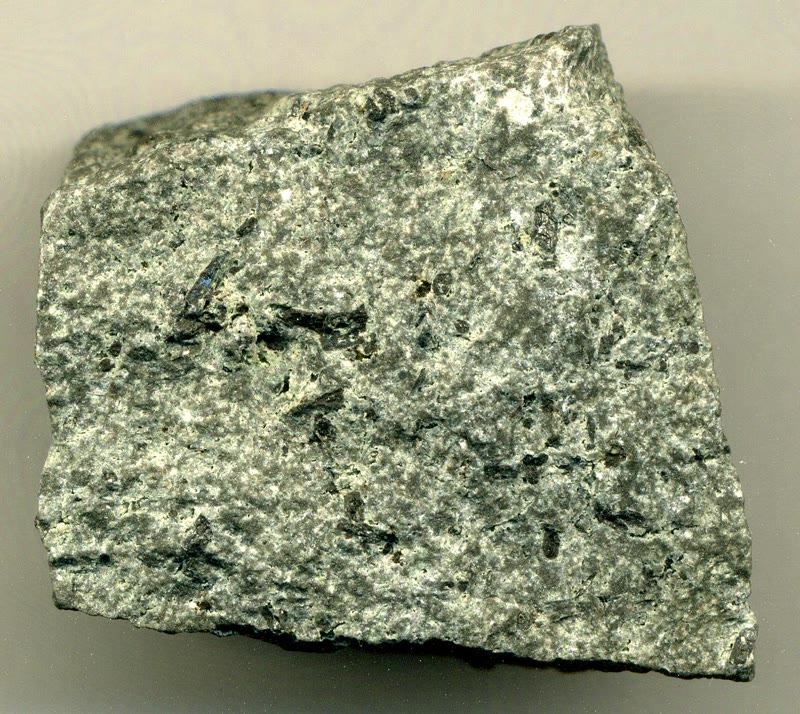
\includegraphics[height=4.4cm]{images/book2/g12-stjohn-andesite.jpg}\hspace{0.03\linewidth}%
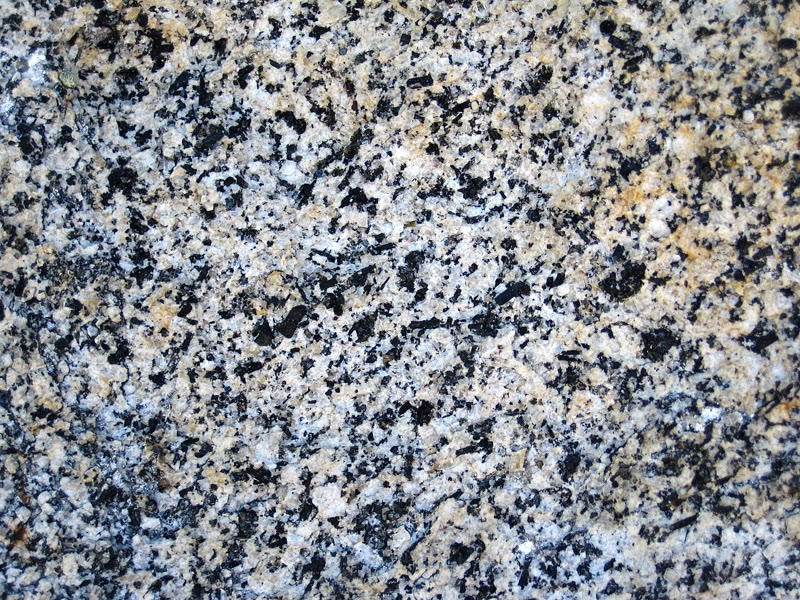
\includegraphics[height=4.4cm]{images/book2/g12-stjohn-granodiorite.jpg}

{\small A la izquierda: \omterm{def:g11:igneous-rocks:rock-names}{andesita}, una \omterm{def:g11:igneous-rocks:volcanic-plutonic}{roca volcánica} de grano fino de los
arcos. A la derecha: \omterm{def:g12:subduction-magmatism:granodiorite}{granodiorita} de Sierra Nevada, con plagioclasa blanca,
cuarzo gris y biotita y hornblenda negras. Fotografías de James St.~John
(CC~BY~2.0).}
\end{omfigure}
% ledger: photo:g12-andesite, photo:g12-granodiorite

Por término medio, la \omterm{def:g12:continental-crust:continental-crust}{corteza continental} superior contiene alrededor de un
\qty{67}{\percent} de \ce{SiO2}: es \omterm{def:g11:igneous-rocks:felsic-mafic}{félsica}, como los granitos que los arcos
producen en abundancia en sus \omterm{def:g12:subduction-magmatism:batholith}{batolitos}.
% ledger: rg14:crust (upper crust SiO2 66.6 wt %), tulane:magma-types, tulane:intrusions

\begin{definition}[Batolito]\label{def:g12:subduction-magmatism:batholith}
Un \emph{batolito}\index{batolito} es una gran masa de \omterm{def:g11:igneous-rocks:volcanic-plutonic}{roca plutónica} que
cubre más de \qty{100}{km^2} donde la erosión la ha dejado al descubierto. Se
forma donde muchos \omterm{def:g11:igneous-rocks:intrusion}{plutones}, intruidos uno tras otro, se unen bajo la
superficie.
\end{definition}
% ledger: earle:batholith, tulane:intrusions

Uno de los mayores del mundo, el Complejo Plutónico de la Costa, recorre la
costa del Pacífico desde la región de Vancouver, en el oeste de Canadá, hasta
el sureste de Alaska. El \omterm{def:g12:subduction-magmatism:batholith}{batolito} de Sierra Nevada, en California, se formó
sobre una \omterm{def:g11:subduction-zones:subduction}{zona de subducción}; la mayoría de sus granitos de Yosemite
cristalizaron en el Cretácico, hace entre 105 y 85 millones de años. Las
rocas que tenían encima se desgastaron a lo largo de millones de años, y los
\omterm{def:g11:igneous-rocks:intrusion}{plutones} que se enfriaron en profundidad forman hoy las montañas.
% ledger: earle:batholith, nps:yosemite, photo:g12-sierra-nevada (St. John description), ics:base.Cretaceous

\begin{omfigure}
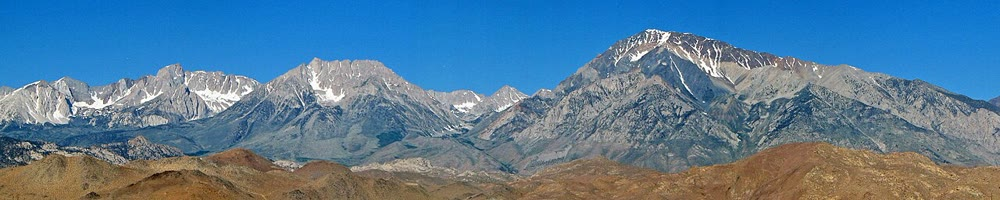
\includegraphics[width=0.94\linewidth]{images/book2/g12-stjohn-sierra-nevada-batholith.jpg}

{\small Sierra Nevada vista desde el este: granito y \omterm{def:g12:subduction-magmatism:granodiorite}{granodiorita} del
\omterm{def:g12:subduction-magmatism:batholith}{batolito} de Sierra Nevada, que cristalizó en profundidad sobre una \omterm{def:g11:subduction-zones:subduction}{zona de
subducción} en el Cretácico. Fotografía de James St.~John (CC~BY~2.0).}
\end{omfigure}
% ledger: photo:g12-sierra-nevada, nps:yosemite

\section{Cómo crecen los continentes}

\begin{definition}[Crecimiento continental]\label{def:g12:subduction-magmatism:continental-growth}
El \emph{crecimiento continental}\index{crecimiento continental} es la
adición de nueva \omterm{def:g12:continental-crust:continental-crust}{corteza continental}, formada a partir del manto, sobre todo
por el magmatismo de los arcos. El crecimiento neto de los continentes es esa
adición menos la \omterm{def:g12:continental-crust:continental-crust}{corteza continental} que vuelve al manto.
\end{definition}
% ledger: sv09:growth, ss09:balance

Los arcos son el lugar donde se forma la roca ligera de los continentes. Las
estimaciones del magma que añaden hoy los arcos son de unos \qty{1.5}{km^3}
al año en los arcos insulares y \qty{1.0}{km^3} al año en los arcos
continentales; promediado a largo plazo, unos \qty{2.7}{km^3} al año. Pero
las \omterm{def:g11:subduction-zones:subduction}{zonas de subducción} también devuelven \omterm{def:g12:continental-crust:continental-crust}{corteza continental} al manto: el
sedimento arrastrado con la \omterm{def:g11:subduction-zones:slab}{losa} y los fragmentos de la placa cabalgante
arrancados por debajo, unos \qty{3.2}{km^3} al año. Las dos cifras son
cercanas, y el crecimiento neto de los continentes en los últimos cientos de
millones de años puede haber sido nulo, o incluso negativo.
% ledger: sv09:growth, ss09:balance

Los continentes también crecen por sus bordes de otro modo. La \omterm{def:g12:continental-crust:continental-crust}{corteza
continental} es demasiado ligera para subducir, así que, cuando una placa lleva
un continente hasta una fosa, los dos continentes quedan soldados en una
colisión (el \cref{ch:g12:mountain-building}). Cada continente tiene un
núcleo antiguo, un \omterm{def:g12:continental-crust:craton}{cratón}, rodeado de cinturones de rocas más jóvenes, las
raíces deformadas de antiguos cinturones montañosos, añadidos uno tras otro
en sus bordes (el \cref{ch:g12:continental-crust}).
% ledger: tulane:no-subduct (continental crust too buoyant to subduct), earle:collision, tulane:cratons

\section{Ejercicios}

\begin{exercise}[$\star$]\label{exo:g12:subduction-magmatism:1}
Da la palabra: (a) una línea de volcanes paralela a una fosa, sobre la placa
que no se hunde; (b) la fusión causada por la adición de agua a una roca;
(c) una \omterm{def:g11:igneous-rocks:volcanic-plutonic}{roca plutónica} con más plagioclasa que feldespato potásico y más de
un \qty{20}{\percent} de cuarzo; (d) una masa de \omterm{def:g11:igneous-rocks:volcanic-plutonic}{roca plutónica} de más de
\qty{100}{km^2}; (e) la adición de nueva \omterm{def:g12:continental-crust:continental-crust}{corteza continental} formada a partir
del manto.
\end{exercise}

\begin{exercise}[$\star$]\label{exo:g12:subduction-magmatism:2}
El 18 de mayo de 1980, la columna de ceniza del monte Santa Helena se elevó a
más de \qty{24}{km} en menos de 15 minutos. (1) ¿Cuál fue su velocidad media
mínima de ascenso, en \unit{km/h} y en \unit{m/s}? (2) Compárala con la
velocidad de la explosión lateral, de al menos \qty{480}{km/h}.
\end{exercise}

\begin{exercise}[$\star$]\label{exo:g12:subduction-magmatism:3}
De los 1214 volcanes del catálogo activos desde el final de la última
glaciación, 838 se alzan sobre una \omterm{def:g11:subduction-zones:subduction}{zona de subducción}. (1) ¿Qué porcentaje es
eso? (2) ¿A qué lado de una fosa están estos volcanes? (3) ¿Por qué no hay
ninguno entre la fosa y el frente volcánico?
\end{exercise}

\begin{exercise}[$\star$]\label{exo:g12:subduction-magmatism:4}
Una roca de grano grueso contiene un \qty{25}{\percent} de cuarzo, un
\qty{45}{\percent} de plagioclasa, un \qty{15}{\percent} de feldespato
potásico y un \qty{15}{\percent} de biotita y hornblenda. (1) ¿Qué fracción
de su feldespato es plagioclasa? (2) ¿Es una \omterm{def:g12:subduction-magmatism:granodiorite}{granodiorita}?
\end{exercise}

\begin{exercise}[$\star$]\label{exo:g12:subduction-magmatism:5}
Da dos razones por las que los volcanes de los arcos tienen erupciones más
explosivas que los de las dorsales.
\end{exercise}

\begin{exercise}[$\star\star$]\label{exo:g12:subduction-magmatism:6}
(1) Un frente volcánico está a \qty{150}{km} de su fosa, sobre una \omterm{def:g11:subduction-zones:slab}{losa} que
buza \ang{35}. ¿A qué profundidad está la \omterm{def:g11:subduction-zones:slab}{losa} bajo él? (2) Compáralo con la
media de \qty{105}{km}.
\end{exercise}

\begin{exercise}[$\star\star$]\label{exo:g12:subduction-magmatism:7}
Supón que la \omterm{def:g11:subduction-zones:slab}{losa} está a \qty{105}{km} bajo todos los frentes volcánicos. ¿A
qué distancia de la fosa está el frente cuando la \omterm{def:g11:subduction-zones:slab}{losa} buza \ang{20}, y cuando
buza \ang{45}? ¿Qué te dice eso sobre dónde buscar el arco?
\end{exercise}

\begin{exercise}[$\star\star$]\label{exo:g12:subduction-magmatism:8}
A \qty{100}{km}, la presión es de unos \qty{3.16}{GPa}. (1) Con $T =
-5.104P^2 + 132.9P + 1120.7$ ($P$ en \unit{GPa}, $T$ en \unit{\celsius}),
calcula la temperatura a la que la \omterm{def:g11:ocean-ridges:peridotite}{peridotita} seca empieza a fundirse allí.
(2) Con agua, empieza a fundirse hacia los \qty{1000}{\celsius}. ¿Cuánto la
rebaja el agua? (3) Supón que la cuña del manto está allí a
\qty{1300}{\celsius}. ¿Se funde en seco? ¿Con agua?
\end{exercise}

\begin{exercise}[$\star\star$]\label{exo:g12:subduction-magmatism:9}
La avalancha de derrubios del monte Santa Helena desplazó unos
\qty{2.5}{km^3} de roca. Los arcos añaden unos \qty{2.7}{km^3} de corteza
nueva al año. (1) ¿Cuántos días del magmatismo de arco de todo el mundo
representa la avalancha? (2) ¿Por qué la comparación es solo una cuestión de
tamaño?
\end{exercise}

\begin{exercise}[$\star\star$]\label{exo:g12:subduction-magmatism:10}
(1) ¿Cuánta corteza nueva añaden los arcos en un millón de años, a
\qty{2.7}{km^3} al año? (2) La \omterm{def:g12:continental-crust:continental-crust}{corteza continental} contiene unos
\qty{9e9}{km^3}. ¿Cuánto tardarían los arcos solos en formar ese volumen, si
no se perdiera nada? (3) Compáralo con la edad de la Tierra, 4500 millones de
años.
\end{exercise}

\begin{exercise}[$\star\star$]\label{exo:g12:subduction-magmatism:11}
(1) En el corte a través de Japón, ¿por qué se dejan fuera muchos terremotos
de menos de \qty{70}{km} de profundidad al ajustar la \omterm{def:g11:subduction-zones:slab}{losa}? (2) Los
terremotos profundos están a \qty{116}{km} de profundidad a \ang{140.5}~E y a
\qty{80}{km} a \ang{141.5}~E, con \qty{86.4}{km} por grado. Calcula el
buzamiento de la \omterm{def:g11:subduction-zones:slab}{losa}.
\end{exercise}

\begin{exercise}[$\star\star\star$]\label{exo:g12:subduction-magmatism:12}
Demuestra que, para un frente a una distancia $d$ de la fosa sobre una \omterm{def:g11:subduction-zones:slab}{losa} de
buzamiento $\theta$, la distancia medida a lo largo de la \omterm{def:g11:subduction-zones:slab}{losa} desde la fosa
hasta el punto situado bajo el frente es $d/\cos\theta$. Para Japón ($d = \qty{270}{km}$, $\theta = \ang{20}$), ¿cuánto mide? La placa del Pacífico se
mueve hacia Japón a unos \qty{83}{mm} al año; tomando esa velocidad a lo
largo de toda la \omterm{def:g11:subduction-zones:slab}{losa}, ¿cuánto tarda un trozo de fondo marino en viajar desde
la fosa hasta debajo de los volcanes?
\end{exercise}
% ledger: usgs:tohoku (83 mm/yr)

\begin{exercise}[$\star\star\star$]\label{exo:g12:subduction-magmatism:13}
La cámara magmática del monte Santa Helena mide unos \qty{1}{km} de anchura y
se extiende desde unos 6 hasta \qty{14}{km} de profundidad. (1) Tratándola
como un cilindro vertical, estima su volumen. (2) Compáralo con los
\qty{2.5}{km^3} de la avalancha. (3) Calcula la \omterm{def:g12:metamorphic-rocks:lithostatic}{presión litostática} en su
techo y en su base ($\rho =
\qty{2830}{kg/m^3}$, $g = \qty{9.81}{m/s^2}$).
\end{exercise}

\begin{exercise}[$\star\star\star$]\label{exo:g12:subduction-magmatism:14}
Los arcos añaden unos \qty{2.7}{km^3} de corteza al año, y las \omterm{def:g11:subduction-zones:subduction}{zonas de
subducción} devuelven unos \qty{3.2}{km^3}. (1) ¿Cuál es el cambio neto por
millón de años? (2) En 500 millones de años, ¿qué fracción de una corteza de
\qty{9e9}{km^3} representa? (3) Los autores califican el crecimiento neto de
``prácticamente nulo''. ¿Por qué, dada la incertidumbre de cada estimación?
\end{exercise}

\begin{exercise}[$\star\star\star$]\label{exo:g12:subduction-magmatism:15}
Un \omterm{def:g12:subduction-magmatism:batholith}{batolito} deja al descubierto \qty{20000}{km^2} de \omterm{def:g12:subduction-magmatism:granodiorite}{granodiorita} cuyos
\omterm{def:g11:igneous-rocks:intrusion}{plutones} se solidificaron entre 5 y \qty{15}{km} de profundidad. (1) Estima
el volumen de magma que representa, suponiéndole \qty{10}{km} de espesor.
(2) A \qty{1}{km^3} al año, el ritmo de todos los arcos continentales del
mundo juntos, ¿cuánto tardarían en formarlo? ¿Qué te dice eso sobre el tiempo
a lo largo del cual se construye un \omterm{def:g12:subduction-magmatism:batholith}{batolito}?
(3) ¿Cuánta roca hubo que erosionar por encima de él antes de que pudiera verse?
\end{exercise}

\begin{problem}[{Problema de fin de semana --- Bajo los volcanes de Japón}]
\label{pb:g12:subduction-magmatism:1}
% ledger: data:b2-usgs-ne-japan, data:gvp, data:pb2002, sa06:slab-depth, hirschmann:solidus, wang20:wet-solidus, earle:arc-water, data:prem
% values (arc_magmatism.py): Megata 139.725, Iwate 141.001, trench 144.12; bins 140.5/141/141.5: 116.4/98.15/80.35 km; P_100km 3.157, dry_T_100km 1489
Los volcanes del noreste de Japón entre \ang{37.5} y \ang{40.5}~N se
encuentran entre \ang{139.7}~E (Megata, el más occidental) y \ang{141.0}~E
(Iwate, el más oriental); la fosa de Japón está a \ang{144.1}~E. La tabla da la
profundidad mediana de los terremotos de más de \qty{70}{km} de profundidad en
tres franjas de longitud, 1976--2025. Toma \qty{111.2}{km} por grado de
latitud.

\begin{center}
\small
\begin{tabular}{|l|c|c|c|}
\hline
longitud (\unit{\degree}~E) & 140.5 & 141.0 & 141.5 \\ \hline
profundidad mediana (\unit{km}) & 116 & 98 & 80 \\ \hline
\end{tabular}
\end{center}

\medskip
\noindent\textbf{Parte I --- El frente volcánico.}
\begin{enumerate}
  \item Demuestra que un grado de longitud a \ang{39}~N mide unos
        \qty{86.4}{km}.
  \item ¿A qué distancia de la fosa está el frente volcánico?
  \item ¿Qué anchura tiene el arco, del Iwate al Megata?
  \item ¿Sobre qué placa se alzan los volcanes, y a qué lado de la fosa?
  \item ¿Por qué no hay volcanes entre la fosa y el Iwate?
\end{enumerate}

\medskip
\noindent\textbf{Parte II --- El corte de los terremotos.}
\begin{enumerate}[resume]
  \item ¿Cuántos kilómetros cambian las profundidades medianas de
        \ang{140.5} a \ang{141.5}~E?
  \item ¿En qué distancia horizontal?
  \item Calcula el buzamiento de la \omterm{def:g11:subduction-zones:slab}{losa}.
  \item Prolonga la recta desde \ang{141.0}~E, \qty{98}{km}, hasta la
        superficie. ¿Dónde la alcanza, y a qué distancia está ese punto de la fosa?
  \item Propón una razón por la que la \omterm{def:g11:subduction-zones:slab}{losa} es menos inclinada cerca de la
        fosa que a más profundidad.
\end{enumerate}

\medskip
\noindent\textbf{Parte III --- La losa bajo los volcanes.}
\begin{enumerate}[resume]
  \item Calcula $H = d\tan\theta$ con la distancia de la pregunta 2 y un
        buzamiento de \ang{20}.
  \item Compáralo con la profundidad mediana bajo el frente.
  \item Compara ambos con el intervalo mundial, de 72 a \qty{173}{km}, y con
        la media, \qty{105}{km}.
  \item ¿A qué profundidad está la \omterm{def:g11:subduction-zones:slab}{losa} bajo el Megata, con la recta de la
        pregunta 9?
  \item Suponiendo que la corteza del arco tiene unos \qty{35}{km} de
        espesor, ¿el techo de la \omterm{def:g11:subduction-zones:slab}{losa} bajo el frente está en la corteza o en
        el manto? ¿A qué distancia por debajo de la base de la corteza?
\end{enumerate}

\medskip
\noindent\textbf{Parte IV --- De dónde viene el agua.}
\begin{enumerate}[resume]
  \item ¿Dónde entró el agua de la \omterm{def:g11:subduction-zones:slab}{losa} en sus rocas, y en qué mineral se
        guarda gran parte de ella?
  \item A \qty{100}{km}, la presión es de unos \qty{3.16}{GPa}. Calcula allí
        el solidus seco con $T = -5.104P^2 + 132.9P + 1120.7$.
  \item Con agua, el solidus está entre 950 y \qty{1000}{\celsius}.
        ¿Cuánto lo rebaja el agua?
  \item ¿Por qué la propia \omterm{def:g11:subduction-zones:slab}{losa} fría no puede ser la fuente del magma?
  \item En resumen: ¿a qué profundidad está la \omterm{def:g11:subduction-zones:slab}{losa} bajo el frente volcánico
        del noreste de Japón?
\end{enumerate}
\end{problem}
